% !TeX program = pdflatex
% !TeX encoding = UTF-8
\documentclass[12pt,a4paper]{article}

\usepackage[utf8]{inputenc}
\usepackage[T1]{fontenc}
\usepackage{lmodern}
\usepackage[brazil]{babel}
\usepackage{listings}
\usepackage{xcolor}
\usepackage{graphicx}
\usepackage{float}
\usepackage{geometry}
\usepackage{indentfirst}
\usepackage{titlesec}
\usepackage{amsmath}
\usepackage{booktabs}
\usepackage{longtable}
\usepackage[hidelinks,pdftitle={Tarefa 11: Particionamento de Dados e Balanceamento de Carga com OpenMP},pdfauthor={Matheus Bezeril Pinto}]{hyperref}

\geometry{a4paper,top=3cm,bottom=2cm,left=3cm,right=2cm}
\setlength{\parindent}{1.25cm}
\setlength{\parskip}{0.2cm}
\setlength{\emergencystretch}{2em}
\titleformat{\section}{\bfseries\large}{\thesection}{1em}{}
\titleformat{\subsection}{\bfseries\normalsize}{\thesubsection}{1em}{}
\graphicspath{{figuras/}}
\renewcommand{\lstlistingname}{Código}
\renewcommand{\lstlistlistingname}{Lista de códigos}
\definecolor{shellFont}{RGB}{233,233,233}
\definecolor{shellBG}{RGB}{44,51,122}
\definecolor{shellKeywords}{RGB}{250,227,0}
\definecolor{shellString}{RGB}{250,166,0}

\lstdefinestyle{Base}{
    basicstyle=\ttfamily\footnotesize,
    numbers=left,numberstyle=\tiny,numbersep=8pt,
    tabsize=4,breaklines=true,breakatwhitespace=false,
    showstringspaces=false,frame=single,
    columns=fullflexible,keepspaces=true,
    inputencoding=utf8,extendedchars=true,
    literate=
    {á}{{\'a}}1 {à}{{\`a}}1 {ã}{{\~a}}1 {â}{{\^a}}1
    {é}{{\'e}}1 {ê}{{\^e}}1 {í}{{\'i}}1
    {ó}{{\'o}}1 {ô}{{\^o}}1 {õ}{{\~o}}1
    {ú}{{\'u}}1 {ç}{{\c{c}}}1
    {Á}{{\'A}}1 {À}{{\`A}}1 {Ã}{{\~A}}1 {Â}{{\^A}}1
    {É}{{\'E}}1 {Ê}{{\^E}}1 {Í}{{\'I}}1
    {Ó}{{\'O}}1 {Ô}{{\^O}}1 {Õ}{{\~O}}1
    {Ú}{{\'U}}1 {Ç}{{\c{C}}}1
}
\lstdefinestyle{CStyle}{
    style=Base,language=C,
    keywordstyle=\color{blue}\bfseries,
    stringstyle=\color{red},
    commentstyle=\color{green!50!black},
    backgroundcolor=\color{gray!10}
}
\lstdefinestyle{Terminal}{
    style=Base,language=bash,
    basicstyle=\ttfamily\footnotesize\color{shellFont},
    keywordstyle=\color{shellKeywords}\bfseries,
    stringstyle=\color{shellString},
    commentstyle=\color{gray!30},
    numberstyle=\tiny\color{black},
    backgroundcolor=\color{shellBG}
}

\title{\textbf{Tarefa 11: Particionamento de Dados e Balanceamento de Carga com OpenMP}}
\author{Matheus Bezeril Pinto}
\date{Outubro de 2026}

\begin{document}
\maketitle

\section*{Resumo}
Este relatório apresenta uma simulação bidimensional de difusão viscosa implementada em C e paralelizada com OpenMP. O modelo retém apenas o termo viscoso da evolução da velocidade, utiliza diferenças finitas no espaço, Euler explícito no tempo e condições de contorno periódicas. A validação considera estados parado, uniforme e com perturbação gaussiana. Para a análise de desempenho, foram comparadas versões com e sem \texttt{collapse(2)}, utilizando os schedules \texttt{static}, \texttt{dynamic,8} e \texttt{guided,8}, com uma, duas e quatro threads solicitadas. Os testes utilizaram uma malha de $400\times400$ células, 5.000 passos e três repetições por configuração, totalizando 54 medições. O menor tempo médio foi de aproximadamente $1{,}762$ s, obtido sem \texttt{collapse(2)}, com quatro threads e \texttt{guided,8}, correspondendo a um speedup de $3{,}267$ sobre a referência comum. O uso de \texttt{collapse(2)} com \texttt{dynamic,8} apresentou custo elevado de escalonamento. Os resultados mostram que a granularidade do trabalho deve ser considerada junto à escolha do schedule.

\section{Introdução}
A paralelização de laços exige identificar quais iterações podem ser executadas de forma independente e como distribuir esse trabalho entre as threads. O OpenMP permite expressar essa distribuição por diretivas e cláusulas, como \texttt{schedule} e \texttt{collapse} \cite{openmp}.

Nesta tarefa, cada célula de uma malha possui duas componentes de velocidade, $u$ e $v$. O estado seguinte de uma célula depende de seu valor atual e de quatro vizinhos. Embora exista dependência entre passos de tempo consecutivos, as células de um mesmo passo podem ser calculadas em paralelo quando os campos de entrada e saída são separados.

O objetivo é verificar a correção dessa evolução e comparar o efeito das diferentes distribuições de trabalho. A implementação foi mantida próxima à versão sequencial em \texttt{Old/}, preservando os modos de inicialização, os diagnósticos e a visualização em Python. Os fontes e os resultados analisados correspondem à revisão \texttt{5192499} do repositório \cite{repositorio}.

\section{Modelo e discretização}
\subsection{Difusão viscosa}
Ao considerar somente os efeitos viscosos com viscosidade cinemática constante $\nu$, o modelo utilizado é
\begin{align}
\frac{\partial u}{\partial t}
 &= \nu\left(\frac{\partial^2u}{\partial x^2}+
                 \frac{\partial^2u}{\partial y^2}\right),\\
\frac{\partial v}{\partial t}
 &= \nu\left(\frac{\partial^2v}{\partial x^2}+
                 \frac{\partial^2v}{\partial y^2}\right).
\end{align}
Não há pressão, forças externas ou transporte advectivo. Assim, trata-se de um modelo de difusão das componentes da velocidade; o programa não resolve o sistema geral de Navier--Stokes nem inclui uma projeção para impor incompressibilidade.

O domínio é $[0,L_x)\times[0,L_y)$, com $L_x=L_y=1$. Para $N_x$ e $N_y$ células, definem-se
\[
\Delta x=\frac{L_x}{N_x},\qquad
\Delta y=\frac{L_y}{N_y}.
\]
A velocidade é associada aos centros das células:
$x_i=(i+1/2)\Delta x$ e $y_j=(j+1/2)\Delta y$.

\subsection{Diferenças finitas e Euler explícito}
Para uma componente genérica $w$, a atualização é
\begin{equation}
\begin{split}
w_{i,j}^{n+1}=w_{i,j}^{n}
 &+r_x\left(w_{i+1,j}^{n}-2w_{i,j}^{n}+w_{i-1,j}^{n}\right)\\
 &+r_y\left(w_{i,j+1}^{n}-2w_{i,j}^{n}+w_{i,j-1}^{n}\right),
\end{split}
\label{eq:atualizacao}
\end{equation}
em que
\[
r_x=\frac{\nu\Delta t}{\Delta x^2},\qquad
r_y=\frac{\nu\Delta t}{\Delta y^2}.
\]
O esquema tem precisão de primeira ordem no tempo e segunda ordem no espaço. Para a difusão explícita em duas dimensões, a condição de estabilidade é
\[
r_x+r_y\leq\frac{1}{2}.
\]
O código define $\nu=0{,}01$, $\alpha=0{,}20$ e
\begin{equation}
\Delta t=\frac{\alpha\min(\Delta x^2,\Delta y^2)}{\nu}.
\end{equation}
Consequentemente, $r_x+r_y\leq 2\alpha=0{,}40$, atendendo à condição inclusive em malhas retangulares.

As condições de contorno são periódicas: o vizinho anterior ao índice zero é o último índice da dimensão, e o vizinho após o último índice é zero. O domínio não possui paredes nem uma fronteira de saída.

\subsection{Condições iniciais}
Os três modos de inicialização são:
\begin{enumerate}
    \item Modo \texttt{0}: $u=v=0$, representando o fluido parado.
    \item Modo \texttt{1}: $u=1$ e $v=0$, representando velocidade uniforme.
    \item Modo \texttt{2}: $v=0$ e
    \[
    u(x,y,0)=1+0{,}5
    \exp\left[-\frac{(x-0{,}5)^2+(y-0{,}5)^2}{2(0{,}08)^2}\right].
    \]
\end{enumerate}
Nos dois primeiros modos, o Laplaciano é nulo e o estado deve permanecer constante. No terceiro, a gaussiana deve se espalhar e perder seu pico. A evolução por difusão não transporta o centro da perturbação como faria um termo advectivo.

\section{Implementação}
\subsection{Organização dos arquivos e da memória}
A implementação divide as responsabilidades em:
\begin{itemize}
    \item \texttt{fluid.h}: parâmetros, estrutura \texttt{Simulation} e protótipos;
    \item \texttt{fluid.c}: alocação, inicialização, condições periódicas, evolução, diagnósticos e gravação;
    \item \texttt{fluid\_sim.c}: seleção do modo e coordenação da execução;
    \item \texttt{visualize\_fluid.py}: leitura dos CSVs e geração do GIF;
    \item \texttt{executar\_testes.sh}: compilação e comparação das configurações OpenMP.
\end{itemize}
Os quatro vetores \texttt{u}, \texttt{v}, \texttt{u\_new} e \texttt{v\_new} são alocados com \texttt{calloc}. A posição $(i,j)$ corresponde ao índice linear $iN_y+j$. Portanto, o laço interno em $j$ percorre posições contíguas de memória.

Durante um passo, os vetores atuais são somente lidos e cada iteração escreve em uma posição distinta dos vetores novos. Não é necessário usar \texttt{atomic} ou \texttt{critical} nessa atualização. Para a carga de $400\times400$, os quatro campos ocupam aproximadamente $5{,}12$ MB, sem contar estruturas e outros custos do processo.

\subsection{Laços paralelos e troca dos campos}
As duas versões são produzidas a partir do mesmo fonte:
\begin{lstlisting}[style=CStyle,caption={Seleção da diretiva OpenMP durante a compilação.}]
#ifdef USE_COLLAPSE
    #pragma omp parallel for collapse(2) schedule(runtime)
#else
    #pragma omp parallel for schedule(runtime)
#endif
    for (int i = 0; i < sim->nx; ++i)
    {
        for (int j = 0; j < sim->ny; ++j)
        {
            /* Leitura dos vizinhos e escrita da celula nova. */
        }
    }
\end{lstlisting}
O trecho acima resume a estrutura dos laços; o corpo completo está na cópia de \texttt{fluid.c} incluída na pasta \texttt{codigos/} do projeto do relatório.

Sem \texttt{collapse}, o espaço distribuído contém $N_x$ iterações, cada uma responsável por uma linha com $N_y$ células. Com \texttt{collapse(2)}, as duas dimensões formam um único espaço lógico com $N_xN_y$ iterações, cada uma correspondente a uma célula.

A opção \texttt{-DUSE\_COLLAPSE} do GCC define a macro \texttt{USE\_COLLAPSE} no pré-processador e seleciona a primeira diretiva. O prefixo \texttt{-D} é uma opção do compilador; não faz parte do nome da macro.

Ao final do \texttt{parallel for}, há uma barreira implícita. Somente depois que todas as células novas estão prontas, \texttt{swap\_fields} troca os ponteiros dos campos atuais pelos novos. Essa troca evita copiar todos os valores e garante que o próximo passo leia um estado completo.

\subsection{Schedules e granularidade}
A cláusula \texttt{schedule(runtime)} seleciona a política em tempo de execução. Ela é definida pela variável \texttt{OMP\_SCHEDULE}, sem recompilação:
\begin{itemize}
    \item \texttt{static}: distribuição estática das iterações; não há obtenção dinâmica de novos blocos durante o laço;
    \item \texttt{dynamic,8}: as threads obtêm blocos de oito iterações conforme terminam o trabalho;
    \item \texttt{guided,8}: os blocos começam maiores e diminuem, com tamanho mínimo de oito, exceto um possível bloco final.
\end{itemize}
O trabalho por célula é essencialmente uniforme. Não há regiões em que uma célula execute um algoritmo mais caro que outra. Portanto, a distribuição dinâmica pode introduzir custo sem necessariamente corrigir um desequilíbrio relevante.

É importante interpretar a unidade do bloco: oito iterações significam oito linhas na versão normal, mas somente oito células na versão com \texttt{collapse(2)}.

\subsection{Medição e modo de desempenho}
A função \texttt{run\_simulation} acumula o tempo apenas do cálculo e da troca dos campos:
\begin{lstlisting}[style=CStyle,caption={Trecho que delimita a medição em cada passo.}]
double inicio = omp_get_wtime();

compute_next_state(sim);
swap_fields(sim);

tempo_calculo += omp_get_wtime() - inicio;
\end{lstlisting}
Esse tempo inclui o custo do paralelismo dentro de \texttt{compute\_next\_state}, como a entrada e a saída da região paralela, o escalonamento e a sincronização. Não inclui a inicialização dos campos, a alocação, os diagnósticos, a gravação de CSVs ou a geração do GIF.

O argumento \texttt{--benchmark} define \texttt{save\_every=0}, desativando frames, metadados de visualização e diagnósticos periódicos. Ele mantém a mesma evolução numérica. A saída ainda informa o tempo de cálculo para que o script o extraia.

\section{Metodologia experimental}
\subsection{Ambiente}
O hardware foi informado como o mesmo utilizado na Tarefa 10. A versão do compilador foi confirmada para os testes da Tarefa 11.
\begin{table}[H]
\centering
\caption{Ambiente informado para as medições.}
\label{tab:ambiente}
\small
\renewcommand{\arraystretch}{1.15}
\begin{tabular}{lp{9cm}}
\toprule
Componente & Especificação\\
\midrule
Processador & Intel Core i5-6400, frequência nominal de 2,70 GHz\\
Núcleos / threads de hardware & 4 núcleos físicos / 4 threads\\
Cache L1d / L1i & 128 KiB / 128 KiB no total, quatro instâncias de cada\\
Cache L2 / L3 & 1 MiB / 6 MiB no total\\
Memória RAM & Aproximadamente 24 GiB\\
Sistema & Ubuntu Linux\\
Compilador & GCC 13.3.0, pacote Ubuntu \texttt{13.3.0-6ubuntu2\string~24.04.1}\\
Opções & \texttt{-O2 -fopenmp}, ligação com \texttt{-lm}\\
\bottomrule
\end{tabular}
\end{table}

Não foram registrados controles de frequência da CPU, carga de outros processos ou afinidade das threads. A frequência nominal não significa frequência constante durante as execuções. Essas condições são consideradas na interpretação da variabilidade.

\subsection{Duas cargas com finalidades diferentes}
A visualização utiliza os parâmetros padrão. O desempenho utiliza uma carga maior para reduzir a influência relativa de medições muito curtas.
\begin{table}[H]
\centering
\caption{Parâmetros das duas cargas analisadas.}
\label{tab:cargas}
\small
\renewcommand{\arraystretch}{1.15}
\begin{tabular}{lrr}
\toprule
Parâmetro & Validação visual & Desempenho\\
\midrule
Modo & 2 & 2\\
Malha & $80\times80$ & $400\times400$\\
Passos & 1.000 & 5.000\\
$\Delta x=\Delta y$ & $0{,}0125$ & $0{,}0025$\\
$\Delta t$ & $0{,}003125$ & $0{,}000125$\\
Tempo físico final & $3{,}125$ & $0{,}625$\\
Atualizações de células & $6{,}4\times10^6$ & $8{,}0\times10^8$\\
Frames & 101, a cada 10 passos & Desativados\\
\bottomrule
\end{tabular}
\end{table}
O segundo caso realiza 125 vezes mais atualizações de células, mas simula um tempo físico menor devido à redução de $\Delta t$. O tempo físico da tabela não é o tempo medido pelo relógio do computador.

\subsection{Configurações e estatísticas}
Foram comparadas duas versões, três quantidades de threads solicitadas $(1,2,4)$ e três schedules, totalizando 18 configurações. Cada configuração foi executada três vezes, gerando 54 medições:
\begin{lstlisting}[style=Terminal,caption={Comando que corresponde à configuração registrada nos resultados.}]
bash executar_testes.sh 2 3 400 400 5000
\end{lstlisting}
O script define \texttt{OMP\_DYNAMIC=FALSE}, solicita o número de threads com \texttt{OMP\_NUM\_THREADS} e aplica cada schedule por \texttt{OMP\_SCHEDULE}. Ele executa as configurações em ordem fixa, sem uma etapa de aquecimento separada. O número efetivo de threads não é gravado nos CSVs.

Para três tempos $T_1,T_2,T_3$, calculam-se
\[
\overline{T}=\frac{1}{3}\sum_{k=1}^{3}T_k,\qquad
s=\sqrt{\frac{1}{2}\sum_{k=1}^{3}(T_k-\overline{T})^2},
\qquad
CV=100\frac{s}{\overline{T}}.
\]
As médias e os speedups são produzidos pelo script original. O desvio padrão amostral e o CV foram calculados adicionalmente para este relatório a partir dos mesmos tempos brutos. Nenhuma medição foi removida.

A referência comum é a média da versão normal com uma thread e \texttt{static}:
\[
T_{\mathrm{ref}}=5{,}755341\;\mathrm{s},\qquad
S=\frac{T_{\mathrm{ref}}}{\overline{T}}.
\]
Esse speedup mede a vantagem sobre uma configuração OpenMP de uma thread, e não sobre um executável sequencial compilado sem OpenMP. A pasta \texttt{Old/} foi usada como referência de correção.

\section{Validação numérica}
Nos modos parado e uniforme, as diferenças entre valores vizinhos são nulas. A Equação~\ref{eq:atualizacao} preserva esses campos. Na verificação da implementação em ambiente de desenvolvimento, os 101 frames dos três modos foram comparados com os da versão sequencial de \texttt{Old/}; as versões normal e com \texttt{collapse(2)} produziram arquivos idênticos para os parâmetros padrão.

Os resultados de campo enviados ao repositório correspondem ao modo 2 na malha de $80\times80$. Os 101 frames dessa execução também coincidem, byte a byte, com os arquivos de referência em \texttt{Old/}. A análise desses frames não encontrou valores não finitos.

\subsection{Decaimento e conservação da média}
Para medir a perturbação no modo 2, utiliza-se $u_{\mathrm{ref}}=1$ e $v_{\mathrm{ref}}=0$:
\[
A_{\max}=\max_{i,j}\sqrt{(u_{i,j}-1)^2+v_{i,j}^2},\qquad
A_{\mathrm{RMS}}=\sqrt{\frac{1}{N_xN_y}
\sum_{i,j}\big[(u_{i,j}-1)^2+v_{i,j}^2\big]}.
\]
\begin{table}[H]
\centering
\caption{Medidas extraídas dos frames inicial e final enviados ao repositório.}
\label{tab:validacao}
\small
\begin{tabular}{lrr}
\toprule
Medida & Inicial & Final\\
\midrule
Máximo da perturbação & $0{,}496958$ & $0{,}046535$\\
RMS da perturbação & $0{,}070898$ & $0{,}022755$\\
Média de $u$ & $1{,}020106193$ & $1{,}020106193$\\
Variância de $u$ & $0{,}004622289$ & $0{,}000113514$\\
Máximo de $|v|$ & $0$ & $0$\\
\bottomrule
\end{tabular}
\end{table}
O máximo e o RMS não crescem entre frames consecutivos, e a variância diminui. A maior variação da média de $u$ ao longo dos arquivos é inferior a $4\times10^{-14}$, compatível com arredondamento numérico e a precisão dos CSVs.

\begin{figure}[H]
\centering
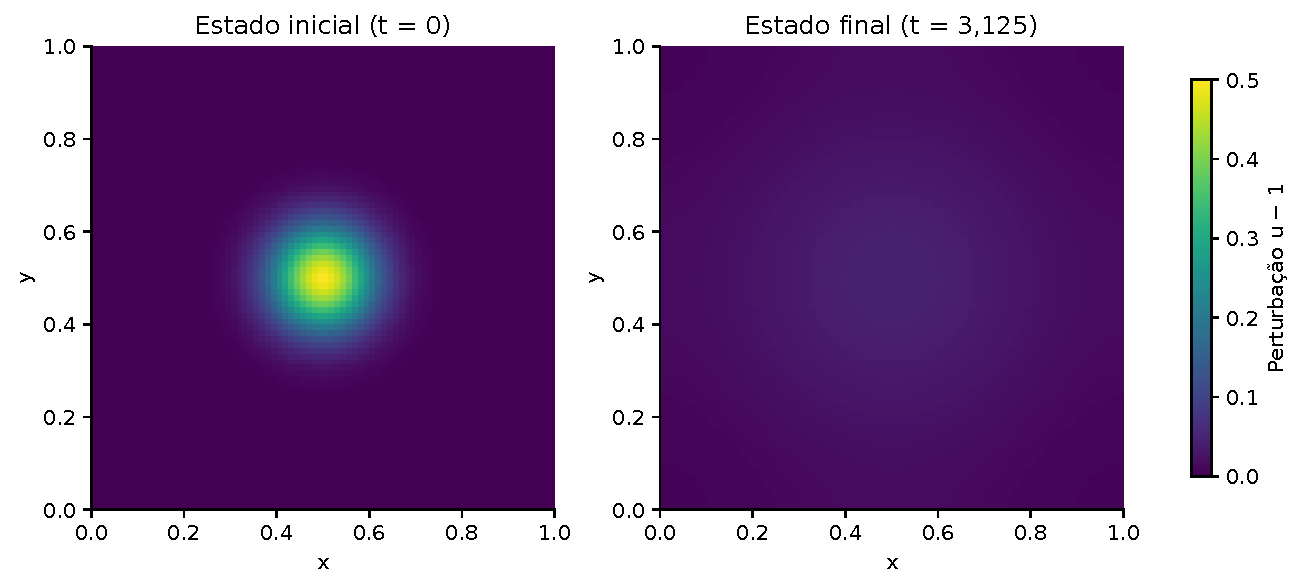
\includegraphics[width=\textwidth]{campos.pdf}
\caption{Perturbação inicial e final na mesma escala de cores, na malha de $80\times80$. A redução do pico e o espalhamento são compatíveis com a difusão.}
\label{fig:campos}
\end{figure}

Sob contornos periódicos, as contribuições dos vizinhos no Laplaciano se cancelam quando somadas sobre todo o domínio. Por isso, a média é conservada. A gaussiana inicial é positiva e acrescenta aproximadamente $0{,}020106193$ à média de $u$; a tendência de longo prazo é um campo uniforme próximo de $u=1{,}020106193$, e não exatamente $u=1$.

Assim, o RMS medido em relação a $u=1$ não precisa tender a zero. A variância em relação à própria média é uma medida complementar da uniformização. O estado final observado ainda não é perfeitamente uniforme.

\begin{figure}[H]
\centering
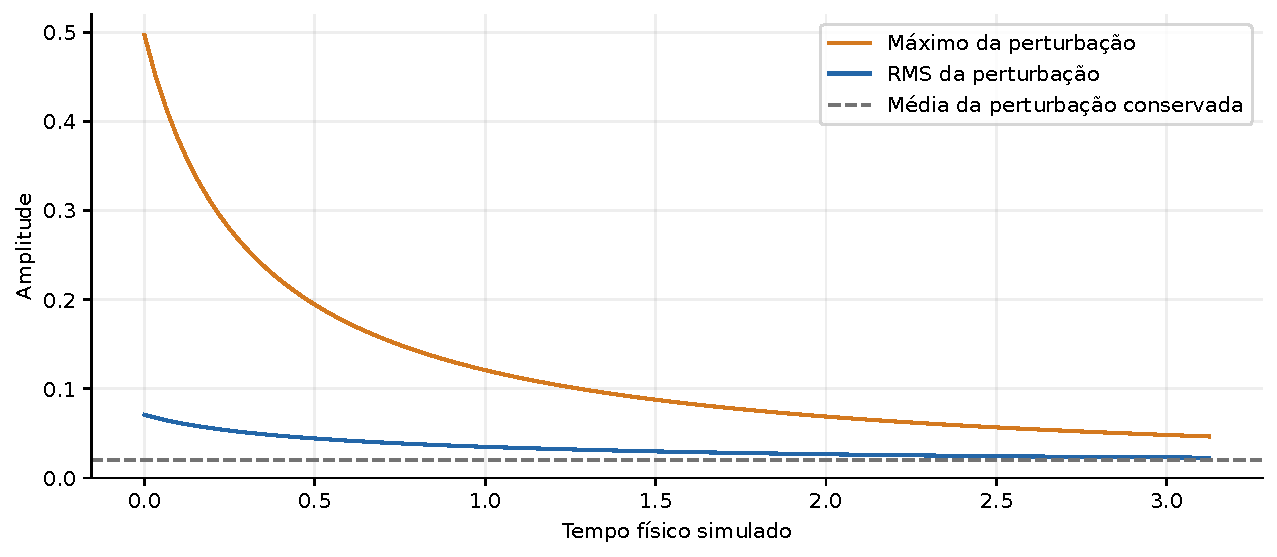
\includegraphics[width=.92\textwidth]{decaimento.pdf}
\caption{Decaimento do máximo e do RMS nos 101 frames. A linha tracejada representa a média positiva da perturbação que é conservada.}
\label{fig:decaimento}
\end{figure}

A concordância com \texttt{Old/} verifica a preservação do comportamento na paralelização. Ela não substitui um estudo de convergência de malha ou a comparação com uma solução analítica, que não fazem parte destes resultados.

\section{Resultados de desempenho}
A Tabela~\ref{tab:resultados} reúne as 18 configurações. A diferença entre os tempos das repetições é mantida no desvio padrão, inclusive nos casos com maior dispersão.
{\small
\setlength{\tabcolsep}{4pt}
\renewcommand{\arraystretch}{1.12}
\begin{longtable}{llrrrrr}
\caption{Resultados da carga de $400\times400$ células e 5.000 passos. $s$ é o desvio padrão amostral; CV é o coeficiente de variação.}\label{tab:resultados}\\
\toprule Versão & Schedule & Threads & Média (s) & $s$ (s) & Speedup & CV (\%) \\
\midrule\endfirsthead
\toprule Versão & Schedule & Threads & Média (s) & $s$ (s) & Speedup & CV (\%) \\
\midrule\endhead
\bottomrule\endfoot
Normal & \texttt{static} & 1 & 5,755 & 0,026 & 1,000 & 0,45 \\
Normal & \texttt{dynamic,8} & 1 & 5,595 & 0,123 & 1,029 & 2,21 \\
Normal & \texttt{guided,8} & 1 & 5,451 & 0,095 & 1,056 & 1,74 \\
Normal & \texttt{static} & 2 & 2,899 & 0,029 & 1,985 & 1,01 \\
Normal & \texttt{dynamic,8} & 2 & 2,907 & 0,020 & 1,980 & 0,68 \\
Normal & \texttt{guided,8} & 2 & 2,801 & 0,020 & 2,055 & 0,73 \\
Normal & \texttt{static} & 4 & 2,054 & 0,420 & 2,801 & 20,43 \\
Normal & \texttt{dynamic,8} & 4 & 1,777 & 0,071 & 3,239 & 3,99 \\
Normal & \texttt{guided,8} & 4 & 1,762 & 0,038 & 3,267 & 2,15 \\
\midrule
Collapse & \texttt{static} & 1 & 6,041 & 0,057 & 0,953 & 0,95 \\
Collapse & \texttt{dynamic,8} & 1 & 9,759 & 0,015 & 0,590 & 0,16 \\
Collapse & \texttt{guided,8} & 1 & 6,099 & 0,028 & 0,944 & 0,45 \\
Collapse & \texttt{static} & 2 & 3,211 & 0,040 & 1,792 & 1,23 \\
Collapse & \texttt{dynamic,8} & 2 & 9,505 & 0,118 & 0,606 & 1,25 \\
Collapse & \texttt{guided,8} & 2 & 3,155 & 0,040 & 1,824 & 1,28 \\
Collapse & \texttt{static} & 4 & 2,225 & 0,347 & 2,587 & 15,59 \\
Collapse & \texttt{dynamic,8} & 4 & 6,890 & 0,226 & 0,835 & 3,28 \\
Collapse & \texttt{guided,8} & 4 & 1,943 & 0,024 & 2,962 & 1,25 \\
\end{longtable}

}
\begin{figure}[H]
\centering
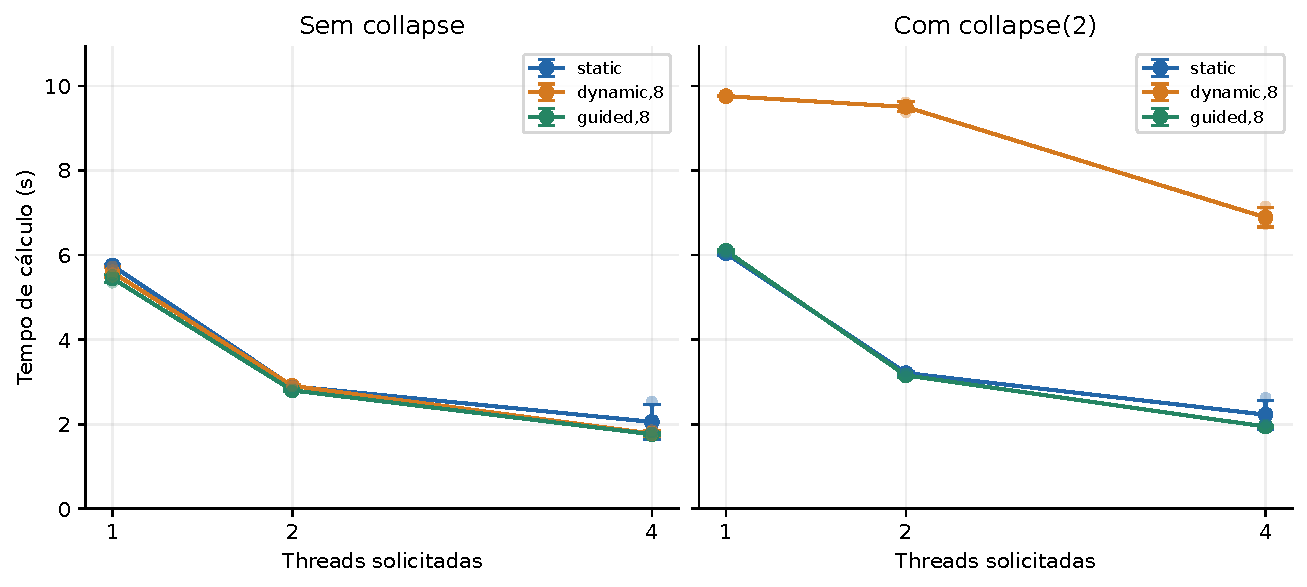
\includegraphics[width=\textwidth]{tempos.pdf}
\caption{Tempos médios por configuração. As barras indicam um desvio padrão amostral e os pontos menores mostram as três medições. Não são intervalos de confiança.}
\label{fig:tempos}
\end{figure}
\begin{figure}[H]
\centering
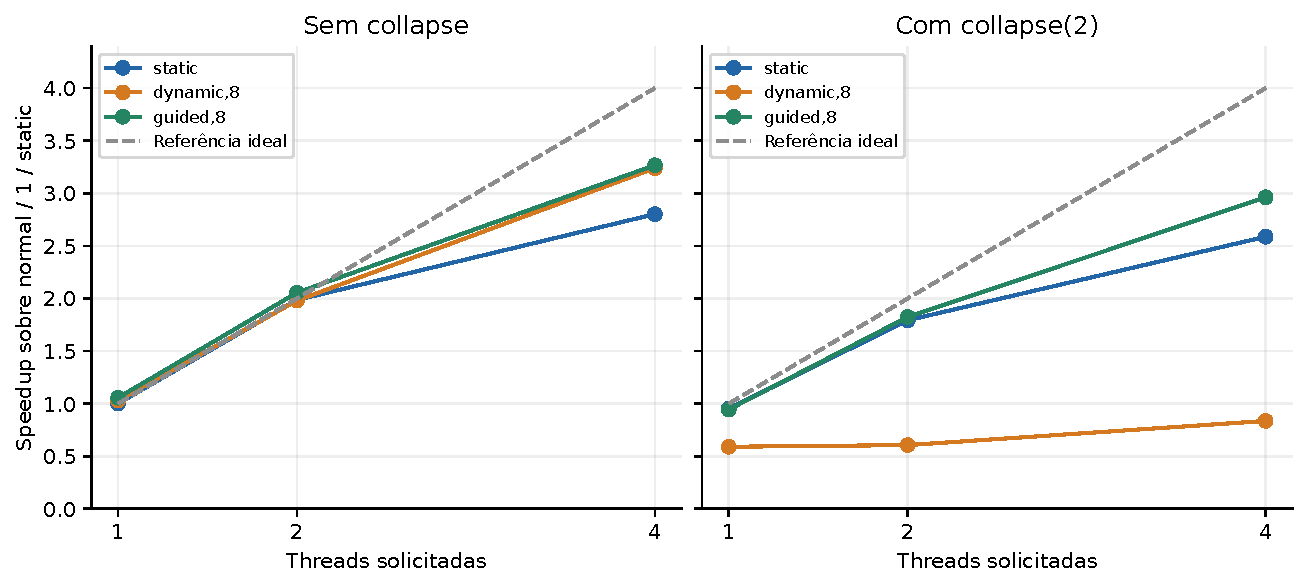
\includegraphics[width=\textwidth]{speedup.pdf}
\caption{Speedup em relação à mesma referência normal / uma thread / \texttt{static}. A linha ideal é uma referência de escala, não um resultado medido.}
\label{fig:speedup}
\end{figure}

O menor tempo médio foi obtido pela versão normal com quatro threads e \texttt{guided,8}: $1{,}761822$ s, com speedup de aproximadamente $3{,}267$. Com \texttt{dynamic,8}, a mesma versão obteve $1{,}777005$ s e speedup de $3{,}239$.

A melhor configuração com \texttt{collapse(2)} também utilizou quatro threads e \texttt{guided,8}, com média de $1{,}943000$ s. Entre as médias deste experimento, nenhuma configuração com \texttt{collapse(2)} superou a configuração normal de mesmo schedule e mesma quantidade de threads.

\section{Discussão}
\subsection{Escalabilidade e referência do speedup}
Sem \texttt{collapse}, \texttt{static} passou de $5{,}755341$ s com uma thread para $2{,}899031$ s com duas, correspondendo a $1{,}985$ vezes de aceleração. Esse resultado é próximo da redução ideal pela metade.

Para a melhor configuração de quatro threads, a razão $S/4$ é aproximadamente $81{,}7\%$ em relação à referência comum. Esse percentual não deve ser confundido com utilização medida da CPU ou com eficiência relativa à versão sequencial de \texttt{Old/}.

O speedup $2{,}055$ observado para duas threads com \texttt{guided,8} não comprova aceleração superlinear, pois a referência usa \texttt{static}. Ao comparar \texttt{guided,8} com seu próprio tempo de uma thread,
\[
\frac{5{,}451358}{2{,}800924}\approx1{,}946.
\]
Portanto, diferenças entre schedules na configuração de uma thread também influenciam os speedups apresentados.

\subsection{Por que \texttt{collapse(2)} não melhorou os tempos}
A malha possui 400 linhas e foram solicitadas no máximo quatro threads. O laço externo já oferece iterações suficientes para a distribuição. Como o cálculo por célula é uniforme, aumentar o espaço lógico de 400 linhas para 160.000 células não cria, por si só, um benefício de balanceamento.

Além disso, o percurso em linhas respeita a disposição contígua dos dados. Alterar o particionamento pode modificar a localidade e os custos de execução. Os tempos confirmam a diferença de desempenho, mas, sem contadores de hardware, não permitem atribuir quantitativamente essa diferença a cache, divisão de índices ou largura de banda de memória.

O resultado não significa que \texttt{collapse} seja sempre inadequado. Ele pode ser útil quando o laço externo oferece poucas iterações em relação à quantidade de threads ou quando combinar as dimensões melhora a distribuição do trabalho.

\subsection{Custo de \texttt{dynamic,8} com \texttt{collapse(2)}}
Na versão normal, um bloco de oito iterações corresponde a oito linhas, ou 3.200 células. Por passo, as 400 linhas formam 50 blocos.

Com \texttt{collapse(2)}, as 160.000 células formam 20.000 blocos de oito células por passo. Ao longo de 5.000 passos, são aproximadamente 100 milhões de blocos, contra 250 mil na versão normal: 400 vezes mais unidades de distribuição.

Essa diferença de granularidade é compatível com o custo elevado observado. A versão com \texttt{collapse(2)} e \texttt{dynamic,8} levou $9{,}759254$ s com uma thread e $6{,}890485$ s com quatro. Há melhora ao aumentar suas próprias threads, mas a configuração de quatro threads continua mais lenta que a referência comum de uma thread.

O \texttt{guided,8} inicia com blocos maiores e reduz o número de obtenções de trabalho muito fino durante boa parte do laço. Isso é coerente com seus tempos menores. A explicação é baseada na política de distribuição e nas medições; não foi feito um perfil interno do runtime para separar cada custo.

\subsection{Variabilidade e limites das conclusões}
As configurações \texttt{static} com quatro threads apresentaram os maiores coeficientes de variação: $20{,}43\%$ na versão normal e $15{,}59\%$ com \texttt{collapse(2)}. Os tempos brutos foram, respectivamente,
\[
(2{,}538934;\;1{,}815439;\;1{,}808791)\ \mathrm{s}
\]
e
\[
(2{,}009164;\;2{,}625166;\;2{,}040834)\ \mathrm{s}.
\]
Os valores mais altos não foram descartados. Podem refletir condições do sistema, frequência ou escalonamento, mas o experimento não registrou evidências para determinar a causa.

A diferença entre \texttt{guided,8} e \texttt{dynamic,8} com quatro threads na versão normal é de aproximadamente $0{,}015$ s, ou $0{,}85\%$. Como essa diferença é pequena diante da dispersão das três amostras, não há base suficiente para afirmar superioridade geral de um deles.

O uso de ordem fixa, a ausência de aquecimento separado e a pequena quantidade de repetições limitam a análise estatística. Ainda assim, as tendências mais marcantes, como o custo de \texttt{dynamic,8} com \texttt{collapse(2)}, aparecem de forma consistente nas amostras.

\section{Conclusão}
A implementação reproduziu o comportamento da versão sequencial nos modos analisados. Na execução com perturbação, o pico e o RMS diminuíram, a média foi conservada e a componente $v$ permaneceu nula, em concordância com o modelo de difusão viscosa com contornos periódicos.

O aumento da carga permitiu obter tempos de segundos e observar aceleração mais clara. A versão normal atingiu speedup de aproximadamente $3{,}267$ com quatro threads, enquanto \texttt{collapse(2)} não melhorou as médias nas condições avaliadas.

O principal aprendizado é que a escolha do schedule depende também da unidade de trabalho. O mesmo tamanho de bloco, oito, passou a significar oito células em vez de oito linhas com o uso de \texttt{collapse(2)}, aumentando muito o custo de distribuição dinâmica. Para este problema e esta quantidade de threads, paralelizar somente o laço externo foi suficiente.

As conclusões se restringem ao hardware, à carga e às amostras apresentados. Como continuidade, seria possível ampliar o número de repetições, controlar a afinidade das threads e variar o tamanho dos blocos dinâmicos, mantendo a mesma referência e a mesma carga.

\appendix
\section{Reprodução das execuções}
Os comandos a seguir são executados na pasta \texttt{Tarefa\_11}. Para gerar os campos e o GIF:
\begin{lstlisting}[style=Terminal]
gcc -O2 -fopenmp fluid_sim.c fluid.c -lm -o fluid_sim
OMP_NUM_THREADS=4 OMP_SCHEDULE=static ./fluid_sim 2

python3 -m venv .venv
source .venv/bin/activate
python -m pip install numpy matplotlib pillow
python visualize_fluid.py
\end{lstlisting}
O ambiente virtual é necessário apenas para as dependências Python. No Ubuntu, o pacote \texttt{python3-venv} deve estar instalado. O programa em C não depende de Python.

Para repetir a comparação de desempenho:
\begin{lstlisting}[style=Terminal]
bash executar_testes.sh 2 3 400 400 5000
\end{lstlisting}
O script recompila as duas versões e grava \texttt{tempos.csv}, \texttt{resumo.csv} e \texttt{configuracao.txt} em \texttt{resultados\_openmp/}. Uma nova execução substitui esses arquivos.

Para compilar manualmente a versão com \texttt{collapse(2)} e testar uma configuração:
\begin{lstlisting}[style=Terminal]
gcc -O2 -fopenmp -DUSE_COLLAPSE \
    -DNX=400 -DNY=400 -DSTEPS=5000 \
    fluid_sim.c fluid.c -lm -o fluid_collapse
OMP_DYNAMIC=FALSE OMP_NUM_THREADS=4 OMP_SCHEDULE=guided,8 \
    ./fluid_collapse 2 --benchmark
\end{lstlisting}

\section{Arquivos que acompanham o relatório}
O projeto LaTeX é independente da posição do restante do repositório. A pasta \texttt{dados/} contém cópias dos três arquivos de desempenho, metadados da visualização, os campos inicial e final, a série de diagnósticos dos 101 frames e as estatísticas derivadas.

A pasta \texttt{codigos/} contém cópias dos cinco fontes analisados. Elas documentam a revisão usada neste relatório e não substituem os fontes principais da tarefa. A função \texttt{compute\_next\_state}, em \texttt{fluid.c}, concentra o cálculo paralelo; \texttt{run\_simulation} delimita a medição, e \texttt{executar\_testes.sh} define a comparação.

O arquivo \texttt{gerar\_figuras.py} recalcula os gráficos e a tabela a partir dos dados incluídos, sem executar uma nova simulação. As figuras e a tabela já estão prontas, de modo que a compilação do \texttt{main.tex} não exige Python, acesso à rede ou autorização de \textit{shell escape}.

\begin{thebibliography}{9}
\bibitem{openmp}
OPENMP ARCHITECTURE REVIEW BOARD.
\textit{OpenMP Application Programming Interface, Version 5.2}.
2021. Disponível em:
\url{https://www.openmp.org/specifications/}.

\bibitem{repositorio}
PINTO, Matheus Bezeril.
\textit{ProgParalela2026.2: Tarefa 11}.
Código e resultados da revisão \texttt{5192499}, 2026.
Disponível em:
\url{https://github.com/39Matheus/ProgParalela2026.2/tree/5192499/Tarefa_11}.
\end{thebibliography}

\end{document}
